\section{Funktioner generelt}
\begin{frame}{Funktioner}
\begin{itemize} 
	\setlength\itemsep{1em}
	\item<1-> En funktion $f$ tildeler ethvert element $x$ i en mængde $X$ præcis ét element $ f(x) $ i en mængde $Y$.
	\item<2-> Mængden $X$ kaldes \emph{domænet} eller \emph{definitionsmængden} for $f$ og mængden $Y$ kaldes \emph{codomænet} for $f$.
	\item<3-> Vi anvender notationen:
	\begin{align*}
	f\colon X\to Y.
	\end{align*}
	\item<4-> Et eksempel på funktioner er $f\colon \R \to [0,\infty[$ givet ved $f(x)=x^2$ og $g\colon ]0,\infty[\to \R$ givet ved $g(x)=e^{\frac{1}{x}}$.
\end{itemize}
\end{frame}

\begin{frame}{Funktioner}
\begin{itemize}
	\item<1-> Figur~\ref{fig:fun11} og Figur~\ref{fig:fun1} viser også eksempler på funktioner.
\end{itemize}
	\begin{figure}[!htbp]
		\begin{minipage}{0.49\textwidth}
			\pgfplotsset{width=0.5\textwidth,compat=1.11}
			\centering
			\begin{tikzpicture}
			\draw \boundellipse{0,0}{0.7}{1.4};
			\draw \boundellipse{3,0}{0.7}{1.4};
			\node[circle,fill,inner sep=1pt] (a) at (0.05,1.0) [label=left:$a$]{};
			\node[circle,fill,inner sep=1pt] (b) at (0.05,0.35) [label=left:$b$]{};
			\node[circle,fill,inner sep=1pt] (c) at (0.05,-0.35) [label=left:$c$]{};
			\node[circle,fill,inner sep=1pt] (d) at (0.05,-1.0) [label=left:$d$]{}; 
			\node[] at (0.45,1.7) [label=left:$X$]{}; 
			\node[circle,fill,inner sep=1pt] (A) at (3.0,0.7) [label=right:$A$]{};
			\node[circle,fill,inner sep=1pt] (B) at (3.0,0.0) [label=right:$B$]{};
			\node[circle,fill,inner sep=1pt] (C) at (3.0,-0.7) [label=right:$C$]{}; 
			\node[] at (3.45,1.7) [label=left:$Y$]{}; 
			\node[] at (1.9,1.3) [label=left:$g$]{}; 
			\draw[->,thick] (a) to (B);
			\draw[->,thick] (b) to (A);
			\draw[->,thick] (c) to (B);
			\draw[->,thick] (d) to(C);
			\end{tikzpicture}
			\caption{En funktion $g$.}
			\label{fig:fun11}
		\end{minipage}
		\begin{minipage}{0.49\textwidth}
			\centering
			\pgfplotsset{width=0.5\textwidth,compat=1.11}
			\centering
			\begin{tikzpicture}
						\draw \boundellipse{0,0}{0.7}{1.4};
			\draw \boundellipse{3,0}{0.7}{1.4};
			\node[circle,fill,inner sep=1pt] at (0.05,1.0) [label=left:$a$]{};
			\node[circle,fill,inner sep=1pt] at (0.05,0.35) [label=left:$b$]{};
			\node[circle,fill,inner sep=1pt] at (0.05,-0.35) [label=left:$c$]{};
			\node[circle,fill,inner sep=1pt] at (0.05,-1.0) [label=left:$d$]{}; 
			\node[] at (0.45,1.7) [label=left:$X$]{}; 
			\node[circle,fill,inner sep=1pt] at (3.0,0.7) [label=right:$A$]{};
			\node[circle,fill,inner sep=1pt] at (3.0,0.0) [label=right:$B$]{};
			\node[circle,fill,inner sep=1pt] at (3.0,-0.7) [label=right:$C$]{}; 
			\node[] at (3.45,1.7) [label=left:$Y$]{}; 
			\node[] at (1.9,1.3) [label=left:$f$]{}; 
			\draw[->,thick] (a) to (A);
			\draw[->,thick] (b) to (A);
			\draw[->,thick] (c) to (C);
			\draw[->,thick] (d) to (C);
			\end{tikzpicture}
			\caption{En funktion $f$.}
			\label{fig:fun1}
		\end{minipage}
	\end{figure}
\end{frame}
\section{Sammensatte funktioner}
\begin{frame}{Funktioner}{Sammensatte funktioner}
\begin{itemize}
		\setlength\itemsep{1em}
	\item<1-> Hvis $f\colon X\to Y$ og $g\colon Y\to Z$ så kan vi definere sammensætningen $g\circ f\colon X\to Z$ ved $(g\circ f)(x)=g(f(x))$.
	\item<8-> Funktionen $f$ kaldes den \emph{indre funktion} og $g$ kaldes den \emph{ydre funktion}.
%	\item Figur~\ref{fig:fun2} viser en skitse af funktionssammensætning.
	\item<9-> Eksempel: Sammensæt $f(x)=\sqrt{x}$ med $g(x)=e^{2x}$.
\end{itemize}

	\begin{figure}[!htbp]
		\pgfplotsset{width=0.5\textwidth,compat=1.11}
		\centering
		\resizebox{8.0cm}{!}{%
		\begin{tikzpicture}
		\draw[visible on = <2->] \boundellipse{0,0}{0.7}{1.4};
		\draw[visible on = <3->] \boundellipse{5,0}{0.7}{1.4};
		\draw[visible on = <5->] \boundellipse{10,0}{0.7}{1.4};
		\node[visible on = <2->] at (0.45,1.7) [label=left:\only<2->{$X$}]{};
		\node[visible on = <3->] at (5.45,1.7) [label=left:\only<3->{$Y$}]{}; 
		\node[visible on = <5->] at (10.45,1.7) [label=left:\only<5->{$Z$}]{}; 
		\node[circle, fill,inner sep=1pt,visible on = <4->] (x) at (0.05,0) [label=left:\only<4->{$x$}]{};
		\node[circle, fill,inner sep=1pt, visible on = <4->] (fx) at (5.05,0) [label=left:\only<4->{$f(x)$}]{};
		\node[circle, fill,inner sep=1pt, visible on = <6->] (gfx) at (10.05,0) [label=left:\only<6->{$g(f(x))$}]{};
		\draw[thick,->,visible on=<4->] (x) to [bend right] node[pos=0.5, label=above:$f$] {} (fx) ;
		\draw[thick,->,visible on=<6->] (fx) to [bend right] node[pos=0.5, label=above:$g$] {} (gfx) ;
		\draw[thick,->,visible on=<7->] (x) to [bend left] node[pos=0.5, label=below:$g\circ f$] {} (gfx) ;
		\end{tikzpicture}%
	}%
%		\caption{En sammensat funktion.}
%		\label{fig:fun2}
	\end{figure}%
\end{frame}

\begin{frame}{Funktioner}{Første-og andengradspolynomier}
\begin{itemize}
		\setlength\itemsep{1em}
	\item<1-> Et førstegradspolynomium er en funktion med forskrift på formen
	\begin{align*}
	f(x)=ax+b.
	\end{align*}
	\item<2-> Grafen for et førstegradspolynomium er en ret linje med hældning $a$ som skærer $y$-aksen i $b$.
	\item<3-> Et andengradspolynomium er en funktion med forskrift på formen
	\begin{align*}
	f(x)=ax^2+bx+c.
	\end{align*}
	\item<4-> Grafen for et andengradspolynomium er en parabel som skærer $y$-aksen i $c$.
	
\end{itemize}
\end{frame}
\section{Første-og andengradspolynomier}
\begin{frame}{Funktioner}{Første-og andengradspolynomier}
\begin{itemize}
	\item<1-> Figur~\ref{fig:fun3} Viser eksempler på første-og andengradspolynomier.
\end{itemize}
\begin{figure}
			\centering
		\resizebox{5.0cm}{!}{%
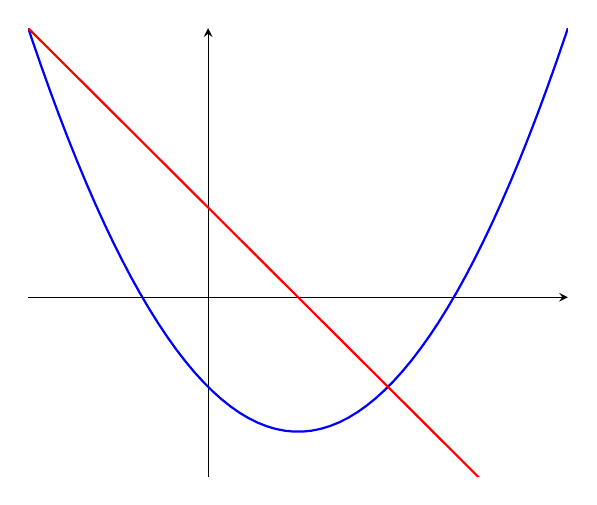
\begin{tikzpicture}
\begin{axis}[xmin=-1,xmax=2,ymin=-2,ymax=3,axis x line=center,
axis y line=center,ticks=none]
\addplot[thick,blue,samples=200]{2*x^2-2*x-1};
\addplot[thick,red,samples=200] {-2*x+1};
\end{axis}
\end{tikzpicture}%
}%
\caption{Grafer for første-og andengradspolynomier.}
\label{fig:fun3}
\end{figure}
\end{frame}

